\documentclass[a4paper,11pt,oneside]{article}

\usepackage[utf8]{inputenc}
\usepackage[a4paper,top=3cm,bottom=3cm,left=3cm,right=3cm]{geometry}
\renewcommand{\familydefault}{\sfdefault}
\usepackage{helvet}
\usepackage[english]{babel}
\usepackage{parskip}
\usepackage[margin=1cm]{caption}
\usepackage{booktabs}
\usepackage[pdftex]{graphicx}
\usepackage[pdftex]{hyperref}
\usepackage{amsmath}
\usepackage{amssymb}
\pdfadjustspacing=1

\newcommand{\mylastname}{Yessengaliyeva}
\newcommand{\myfirstname}{Merey}
\newcommand{\mynumber}{30006199}
\newcommand{\myname}{\myfirstname{} \mylastname{}}
\newcommand{\mytitle}{Ontology-Guided Hybrid Causal Discovery in ESG Data: LLM-Based Development of Query Interface}
\newcommand{\mysupervisor}{Prof.~Dr.~Hendro Wicaksono}

\hypersetup{
  pdfauthor = {\myname},
  pdftitle = {\mytitle},
  pdfkeywords = {ESG, ontology, causal discovery, SPARQL, LLM, ESGOnt},
  colorlinks = {true},
  linkcolor = {blue}
}

\begin{document}
  \pagenumbering{roman}

  \thispagestyle{empty}

  \begin{flushright}
    \includegraphics[scale=0.8]{bsc-logo}
  \end{flushright}
  \vspace*{40mm}
  \begin{center}
    \huge
    \textbf{\mytitle}
  \end{center}
  \vspace*{4mm}
  \begin{center}
   \Large by
  \end{center}
  \vspace*{4mm}
  \begin{center}
    \LARGE
    \textbf{\myname}
  \end{center}
  \vspace*{20mm}
  \begin{center}
    \Large
    Bachelor Thesis \\[2ex]
    Computer Science
  \end{center}
  \vfill
  \begin{flushleft}
    \large
    Submission: May 2026 \hfill Supervisor: \mysupervisor \\
    \rule{\textwidth}{1pt}
  \end{flushleft}
  \begin{center}
    School of Computer Science and Engineering, Constructor University
  \end{center}

  \newpage
  \thispagestyle{empty}

  \begin{center}
    \Large \textbf{Statutory Declaration}
    \vspace*{8mm}
  \end{center}

  \begin{center}
    \begin{tabular}{|l|p{85mm}|}
      \hline
      Family Name, Given/First Name & \mylastname, \myfirstname \\
      Matriculation number & \mynumber \\
      Kind of thesis submitted & Bachelor Thesis \\
      \hline
    \end{tabular}
    \vspace*{8mm}
  \end{center}

  \subsection*{English: Declaration of Authorship}

  I hereby declare that the thesis submitted was created and written solely by myself without any external support. Any sources, direct or indirect, are marked as such. I am aware of the fact that the contents of the thesis in digital form may be revised with regard to the usage of unauthorized aid as well as whether the whole or parts of it may be identified as plagiarism. I do agree my work to be entered into a database for it to be compared with existing sources, where it will remain in order to enable further comparisons with future theses. This does not grant any rights of reproduction and usage, however.

  This document was neither presented to any other examination board nor has it been published.

  \subsection*{German: Erklärung der Autorenschaft (Urheberschaft)}

  Ich erkläre hiermit, dass die vorliegende Arbeit ohne fremde Hilfe ausschließlich von mir erstellt und geschrieben worden ist. Jedwede verwendeten Quellen, direkter oder indirekter Art, sind als solche kenntlich gemacht worden. Mir ist die Tatsache bewusst, dass der Inhalt der Thesis in digitaler Form geprüft werden kann im Hinblick darauf, ob es sich ganz oder in Teilen um ein Plagiat handelt. Ich bin damit einverstanden, dass meine Arbeit in einer Datenbank eingegeben werden kann, um mit bereits bestehenden Quellen verglichen zu werden und dort auch verbleibt, um mit zukünftigen Arbeiten verglichen werden zu können. Dies berechtigt jedoch nicht zur Verwendung oder Vervielfältigung.

  Diese Arbeit wurde noch keiner anderen Prüfungsbehörde vorgelegt noch wurde sie bisher veröffentlicht.

  \vspace{20mm}

  \dotfill\\
  Date, Signature

  \newpage

  \section*{Abstract}

This thesis presents an ontology-guided hybrid causal discovery framework for ESG (Environmental, Social, and Governance) data, coupled with a Large Language Model (LLM)-based natural language query interface. The framework integrates ESGOnt with the PC causal discovery algorithm and applies ontology-derived directional constraints to reduce semantically implausible causal interpretations. In parallel, a query interface powered by the Groq API (LLaMA 3.3) translates user questions into SPARQL queries executed against ESGOnt, improving accessibility for non-technical users. The prototype is implemented as a Gradio web application. In controlled synthetic experiments (3,000 observations), the baseline PC model achieves precision 0.889 and recall 1.000, while ontology constraints provide an explicit semantic filtering layer. A real-world ESG banking pilot (110 raw records, 71 model-ready rows after preprocessing) is additionally used to assess practical feasibility under noisy and heterogeneous reporting conditions. Overall, results support the practical complementarity of ontology priors and statistical causal discovery, while highlighting the need for expanded real-data validation and benchmark-level NL2SPARQL evaluation.

  \newpage
  \tableofcontents

  \clearpage
  \pagenumbering{arabic}

% ========================
\section{Introduction}
% ========================

\subsection{Background}

Environmental, Social, and Governance (ESG) criteria have become central to modern corporate accountability and investment decision-making. Over the past decade, institutional investors, regulators, and corporate stakeholders have increasingly relied on ESG metrics to assess non-financial risks and long-term sustainability of organizations. As regulatory frameworks such as the European Sustainability Reporting Standards (ESRS), the Global Reporting Initiative (GRI), and the Task Force on Climate-related Financial Disclosures (TCFD) increasingly require structured ESG disclosures, organizations face growing pressure to not only report ESG metrics but also to understand the causal relationships between them.

Understanding these relationships goes beyond simple correlation. For example, does improving board diversity causally reduce corruption cases, or do they merely co-occur? Does reducing greenhouse gas emissions lead to improved financial performance, or is the relationship confounded by industry-level factors? Answering such questions requires causal inference — the systematic identification of cause-and-effect relationships from data — rather than descriptive statistics alone.

At the same time, the semantic representation of ESG knowledge has advanced significantly through ontology-based approaches. ESGOnt \cite{wicaksono2022} is an OWL-based ontology that formalizes ESG concepts, their categories, and relationships aligned with GRI, SASB, and SDG frameworks. Such ontologies encode domain knowledge that can serve as a powerful prior for guiding data-driven analysis — yet their integration with causal discovery methods remains largely unexplored.

\subsection{Problem Statement}

Despite the availability of ESG ontologies and causal discovery methods, several challenges remain unaddressed. First, purely data-driven causal discovery methods — such as the PC algorithm or LiNGAM — operate without domain knowledge and may produce semantically invalid causal relationships. For instance, a statistical method might suggest that carbon intensity causes CO$_2$ emissions, when in fact carbon intensity is mathematically derived from emissions data. Such spurious directions are statistically plausible but domain-invalid, and purely data-driven methods cannot rule them out.

Second, ESG ontologies such as ESGOnt encode rich domain knowledge about the hierarchical structure of ESG concepts and their relationships, but this knowledge is typically used only for semantic querying and classification — not for constraining causal discovery. The potential for ontology-derived constraints to improve the semantic validity of causal graphs has not been systematically explored.

Third, even when valid ESG knowledge graphs exist, they remain inaccessible to business users who lack the technical expertise to formulate SPARQL queries. Natural language interfaces powered by Large Language Models (LLMs) offer a promising solution, but their application to ESG ontologies has not been demonstrated in combination with causal discovery systems.

\subsection{Objectives}

This thesis addresses these gaps by developing an ontology-guided hybrid causal discovery system for ESG data, coupled with a natural language query interface powered by a Large Language Model. Specifically, the thesis pursues the following objectives:

\begin{enumerate}
    \item To integrate ESGOnt ontological constraints into the PC causal discovery algorithm as forbidden edge constraints, improving the semantic validity of discovered causal graphs.
    \item To develop an LLM-based natural language query interface that automatically translates user questions into SPARQL queries executed against the ESGOnt knowledge base.
    \item To evaluate the proposed system in two settings: (i) synthetic ESG data with known ground truth for quantitative causal metrics, and (ii) a real-world ESG banking dataset to assess feasibility under practical data limitations.
    \item To define and report evaluation metrics beyond skeleton-level F1, including semantic validity and orientation quality.
    \item To deploy a functional prototype as a Gradio web application accessible to non-technical business users.
\end{enumerate}

\subsection{Contributions}

The main contributions of this work are:

\begin{itemize}
    \item A hybrid causal discovery pipeline integrating the PC algorithm with ESGOnt-derived forbidden edge constraints, demonstrating qualitative improvement in semantic validity over purely data-driven baselines.
    \item An LLM-based natural language query interface using the Groq API (LLaMA 3.3) to translate user questions into SPARQL queries over ESGOnt, accompanied by a benchmark protocol for NL2SPARQL evaluation.
    \item A synthetic ESG dataset of 3,000 observations with embedded ground truth causal structure, plus a real-world ESG banking dataset pilot (110 samples, 12 numeric features after preprocessing) for feasibility assessment.
    \item A Gradio-based prototype demonstrating the full integrated system for business users, combining ontology querying and causal graph visualization.
\end{itemize}

\subsection{Thesis Structure}

The remainder of this thesis is organized as follows. Section~2 reviews related work on ESG ontologies, causal discovery methods, and natural language interfaces for knowledge graphs. Section~3 describes the system architecture and methodology, including the hybrid causal discovery pipeline and the LLM-based query interface. Section~4 presents the experimental setup, including the synthetic dataset generation and evaluation configuration. Section~5 discusses the results of the causal discovery experiments and query interface evaluation. Section~6 concludes with a summary of findings and directions for future work.

% ========================
\section{Background and Related Work}
% ========================

\subsection{ESG Data and Ontologies}

Environmental, Social, and Governance (ESG) reporting has grown significantly over the past decade, driven by regulatory frameworks such as the Global Reporting Initiative (GRI), the Task Force on Climate-related Financial Disclosures (TCFD), and the European Sustainability Reporting Standards (ESRS). These frameworks define standardized indicators across three domains: environmental performance, social responsibility, and corporate governance. ESG datasets are typically high-dimensional, heterogeneous, and subject to inconsistent reporting standards, making automated analysis and causal inference particularly challenging.

To support structured representation of ESG knowledge, ontology-based approaches have been proposed. An ontology is a formal, machine-readable specification of concepts, categories, and relationships within a domain \cite{gruber1993}. ESGOnt \cite{wicaksono2022} is an OWL-based ontology that formalizes ESG concepts aligned with GRI, SASB, and SDG frameworks, organizing knowledge into three top-level domains — Environmental, Social, and Governance — each containing multiple categories and performance indicators. ESGOnt also encodes relationships between concepts via OWL object properties such as \texttt{contributesTo} and \texttt{hasCause}, capturing expert knowledge about plausible and implausible causal directions.

\subsection{Causal Discovery Methods}

Causal discovery refers to the automated identification of causal relationships from observational data. Unlike correlation analysis, causal discovery aims to recover the underlying causal structure in the form of a Directed Acyclic Graph (DAG), where nodes represent variables and directed edges represent causal influences. The field has grown significantly since the foundational work of Pearl \cite{pearl2000} and Spirtes et al. \cite{spirtes2000}, who established the theoretical foundations for causal reasoning from observational data.

Existing causal discovery methods can be broadly categorized into three families.

\textbf{Constraint-based methods}, such as the PC algorithm \cite{spirtes2000} and FCI (Fast Causal Inference), use conditional independence tests to determine the skeleton of the causal graph and then apply orientation rules to direct edges. The PC algorithm operates in two phases: first constructing an undirected skeleton by removing edges between variables that are conditionally independent given some subset of other variables, then orienting edges using Meek's orientation rules to produce a Completed Partially Directed Acyclic Graph (CPDAG). For continuous data under linear-Gaussian assumptions, Fisher's Z test is commonly used for conditional independence testing.

\textbf{Score-based methods}, such as GES (Greedy Equivalence Search) \cite{hauser2012} and NOTEARS, search over the space of DAGs by optimizing a goodness-of-fit score such as the Bayesian Information Criterion (BIC). These methods are generally more computationally expensive than constraint-based methods but can be more robust in low-sample settings.

\textbf{Functional causal model methods}, such as LiNGAM \cite{shimizu2006}, assume specific functional forms for the causal relationships and exploit properties of the noise distribution to identify unique causal directions. LiNGAM assumes linear relationships with non-Gaussian noise, enabling full identification of the causal DAG rather than only the equivalence class. This makes it particularly powerful when the data distribution deviates from Gaussianity.

\subsubsection{Background Knowledge Integration}

A key limitation of purely data-driven causal discovery is that statistical methods alone cannot distinguish between Markov-equivalent causal structures — DAGs that encode the same conditional independence relationships but differ in edge directions. This means that even with infinite data, some causal directions cannot be determined from observational data alone.

To address this limitation, several causal discovery frameworks support the integration of background knowledge as prior constraints. The PC algorithm, for example, allows users to specify \textit{forbidden edges} (pairs of variables that cannot be directly causally connected) and \textit{required edges} (pairs that must be causally connected). These constraints are enforced during the orientation phase, restricting the search space to causally plausible structures.

Prior knowledge for causal discovery has traditionally been provided manually by domain experts. However, this process is time-consuming, requires deep domain expertise, and does not scale to high-dimensional datasets. Automated extraction of causal constraints from domain knowledge bases — such as ontologies — offers a promising alternative that combines the scalability of data-driven methods with the semantic validity of expert knowledge.

\subsubsection{Causal Discovery in ESG Data}

The application of causal discovery to ESG data is a relatively emerging area. Several studies have explored causal relationships between ESG indicators and financial performance, typically using Granger causality or structural equation models. However, these approaches require strong assumptions about functional form and variable ordering, and do not leverage structured domain knowledge from ESG ontologies.

To the best of our knowledge, this thesis represents one of the first attempts to integrate ESGOnt ontological constraints directly into a causal discovery algorithm for ESG data, combining the semantic richness of the ontology with the statistical power of constraint-based causal discovery.

\subsection{Natural Language Interfaces for Knowledge Graphs}

Knowledge graphs and ontologies are typically queried using formal languages such as SPARQL (SPARQL Protocol and RDF Query Language). SPARQL is a powerful query language that enables complex pattern matching over RDF triples, supporting SELECT, CONSTRUCT, ASK, and DESCRIBE query forms. However, constructing valid SPARQL queries requires substantial technical expertise — including knowledge of the ontology's namespace, class hierarchy, and property names — creating a significant barrier for domain experts and business users.

Natural Language Interfaces (NLI) for knowledge graphs aim to bridge this gap by automatically translating user questions expressed in natural language into formal queries \cite{hoffner2017}. The NL2SPARQL task has been studied extensively in the semantic web community, with benchmark datasets such as QALD (Question Answering over Linked Data) and LC-QuAD used to evaluate system performance.

\subsubsection{Traditional and Neural Approaches}

Early NLI approaches relied on rule-based parsing and template matching, mapping question patterns to predefined SPARQL templates. While effective for narrow domains with well-defined question types, these approaches lack generalization and require significant manual engineering for each new ontology.

More recent methods leverage neural sequence-to-sequence models trained end-to-end on NL-SPARQL pairs. These models learn to translate natural language questions into SPARQL queries without explicit rule engineering, generalizing better across question types. However, they require large amounts of training data and may struggle with ontologies not represented in the training set.

\subsubsection{LLMs for NL2SPARQL}

The emergence of Large Language Models (LLMs) such as GPT-4, Gemini, and LLaMA has significantly advanced the state of NL2SPARQL. LLMs trained on vast corpora of text and code have demonstrated strong performance on structured query generation tasks, including SQL and SPARQL generation, particularly when provided with schema or ontology context in the prompt \cite{omar2023}.

The key advantage of LLM-based approaches is their ability to generate syntactically valid queries for previously unseen ontologies through in-context learning — providing the ontology structure in the prompt without any fine-tuning. This makes them particularly suitable for domain-specific ontologies such as ESGOnt, for which no NL-SPARQL training data exists.

Recent work has shown that LLMs can effectively generate SPARQL queries when the prompt includes the ontology namespace, key class definitions, and example queries \cite{omar2023}. Prompt engineering strategies such as chain-of-thought prompting and few-shot examples further improve query generation accuracy.

In this thesis, the Groq API (LLaMA 3.3) is used to generate SPARQL queries over ESGOnt based on user questions. The LLM receives a structured prompt containing the ontology prefix, key class hierarchies, and query generation instructions. The generated SPARQL query is then executed against the ESGOnt knowledge base using the \texttt{rdflib} library in Python, and results are returned to the user through a Gradio-based interface. This approach eliminates the need for users to understand SPARQL syntax while ensuring that answers are grounded strictly in the ontology, avoiding the hallucination problem common in open-ended LLM responses.

\subsection{Research Gap and Novelty}

The review of related work reveals a clear research gap at the intersection of three areas: ESG ontologies, causal discovery, and natural language interfaces. Existing approaches either (1) use ESG ontologies purely for knowledge representation and semantic querying without causal analysis, (2) apply causal discovery to ESG data without leveraging ontological domain knowledge, or (3) develop natural language interfaces for general knowledge graphs without integration with causal discovery systems.

This thesis addresses this gap by proposing a unified system that combines all three components: ontology-derived causal constraints improve the semantic validity of discovered causal graphs, while an LLM-based query interface makes both the ontology and the causal discovery results accessible to non-technical business users. The novelty lies in the automated extraction of forbidden edge constraints from ESGOnt and their integration into the PC algorithm, replacing manual constraint formulation with a systematic, ontology-driven approach.

% ========================
\section{Methodology}
% ========================

\subsection{System Architecture}

The proposed system consists of two main components: (1) an LLM-based natural language query interface for ESGOnt, and (2) an ontology-guided hybrid causal discovery pipeline. Both components share the ESGOnt ontology as a common knowledge base, ensuring that the query interface and the causal discovery pipeline operate on the same semantic foundation.

The query interface accepts a user question in natural language, forwards it to the Groq API (LLaMA 3.3) with a structured prompt containing ESGOnt class definitions, receives a generated SPARQL query, executes it against the ESGOnt knowledge base using \texttt{rdflib}, and returns the result to the user via a Gradio web interface. The causal discovery pipeline loads ESG tabular data, extracts ontological constraints from ESGOnt as forbidden causal edges via SPARQL queries, runs the PC algorithm with and without these constraints, and outputs causal graphs for comparison and evaluation.

The two components are designed to be complementary: the query interface allows users to explore the ontology structure and understand the domain knowledge, while the causal discovery pipeline uses that same domain knowledge to produce semantically valid causal graphs from data. Together, they form a unified system for ESG knowledge exploration and causal analysis.

\subsection{ESGOnt Ontology}

ESGOnt is an OWL-based ontology loaded via \texttt{rdflib} containing 604 RDF triples. The ontology is serialized in RDF/XML format and follows the OWL 2 DL profile, enabling both semantic reasoning and SPARQL querying. The ontology namespace is \texttt{http://www.annasvijaya.com/ESGOnt/esgontology\#}, abbreviated as \texttt{esg:} throughout this thesis.

\subsubsection{Ontology Structure}

ESGOnt defines three top-level domain classes: \texttt{esg:Environmental}, \texttt{esg:Social}, and \texttt{esg:Governance}, each declared as a subclass of \texttt{esg:Domain}. Each domain contains multiple category subclasses declared under \texttt{esg:Category}. For example:

\begin{itemize}
    \item \textbf{Environmental categories:} \texttt{esg:GHG\_Emissions}, \texttt{esg:Energy}, \texttt{esg:Water}, \texttt{esg:Waste}, \texttt{esg:Biodiversity}
    \item \textbf{Social categories:} \texttt{esg:Labor\_Practices}, \texttt{esg:Human\_Rights}, \texttt{esg:Health\_and\_Safety}, \texttt{esg:Community}
    \item \textbf{Governance categories:} \texttt{esg:Board\_Diversity}, \texttt{esg:Corruption}, \texttt{esg:Transparency}, \texttt{esg:Shareholder\_Rights}
\end{itemize}

The ontology also defines object properties encoding relationships between concepts, including \texttt{contributesTo}, \texttt{hasCause}, \texttt{hasCategory}, \texttt{consumesEnergy}, \texttt{consumesWater}, \texttt{generatesWaste}, and \texttt{belongsToCategory}. These properties capture domain knowledge about how ESG concepts relate to each other and are used to derive causal constraints.

\subsubsection{Ontological Constraint Extraction}

Causal constraints are extracted from ESGOnt using SPARQL queries executed via \texttt{rdflib}. The constraint extraction process identifies pairs of variables where ontological semantics imply a forbidden causal direction. Specifically, four forbidden edges are derived based on the following domain reasoning:

\begin{enumerate}
    \item \textbf{\texttt{carbon\_intensity} $\not\rightarrow$ \texttt{co2\_emissions}:} Carbon intensity is defined as GHG emissions normalized by an output metric (e.g., revenue or production volume). It is mathematically derived from CO$_2$ emissions and therefore cannot causally precede them. ESGOnt encodes carbon intensity as a derived indicator under \texttt{esg:GHG\_Emissions}, making the reverse direction semantically invalid.

    \item \textbf{\texttt{corruption\_cases} $\not\rightarrow$ \texttt{board\_diversity}:} ESGOnt places \texttt{Board\_Diversity} as a structural governance property that determines the composition of corporate decision-making bodies. Board diversity influences corporate culture and ethical outcomes, including corruption. The reverse direction — that corruption cases cause board diversity — is semantically invalid under ESGOnt's governance model.

    \item \textbf{\texttt{injury\_frequency\_rate} $\not\rightarrow$ \texttt{turnover\_rate}:} High employee turnover leads to less experienced workers and inadequate safety training, which in turn increases workplace injury rates. ESGOnt's \texttt{Health\_and\_Safety} and \texttt{Labor\_Practices} categories encode this directional relationship, making the reverse direction domain-invalid.

    \item \textbf{\texttt{green\_financing} $\not\rightarrow$ \texttt{governance\_compliance\_score}:} Governance compliance is a prerequisite for accessing green financing instruments such as green bonds and sustainability-linked loans. ESGOnt encodes governance compliance as a structural property that enables sustainable finance activities, making the reverse causal direction implausible.
\end{enumerate}

\subsection{Hybrid Causal Discovery Pipeline}

The hybrid causal discovery pipeline is implemented in Python using the \texttt{causal-learn} library and operates in two modes: baseline and ontology-guided.

\subsubsection{Data Preprocessing}

The ESG dataset is loaded from a CSV file containing 3,000 observations and 10 numeric variables. All variables are standardized to zero mean and unit variance prior to causal discovery, as the Fisher-Z test assumes linearity and the PC algorithm's performance can be sensitive to scale differences between variables. Missing values, if present, are imputed using column means.

\subsubsection{Baseline PC Algorithm}

In the baseline mode, the PC algorithm is applied directly to the standardized ESG dataset using Fisher-Z conditional independence tests at a significance level of $\alpha = 0.05$. The algorithm proceeds in two phases:

\begin{enumerate}
    \item \textbf{Skeleton construction:} Starting from a complete undirected graph, edges are removed between variable pairs that are conditionally independent given some subset of the remaining variables. The significance level $\alpha$ controls the threshold for independence — lower values produce sparser graphs.

    \item \textbf{Edge orientation:} The remaining undirected edges are oriented using Meek's rules, first identifying v-structures (colliders) of the form $X \rightarrow Z \leftarrow Y$ where $X$ and $Y$ are not adjacent, then propagating orientations to avoid cycles and additional v-structures.
\end{enumerate}

The output is a Completed Partially Directed Acyclic Graph (CPDAG), where some edges may remain undirected due to Markov equivalence. The CPDAG is converted to an adjacency matrix for evaluation against the ground truth structure.

\subsubsection{Ontology-Guided PC Algorithm}

In the ontology-guided mode, the four forbidden edges derived from ESGOnt are applied as post-processing constraints to the CPDAG produced by the baseline PC algorithm. Specifically, for each forbidden edge $A \not\rightarrow B$, if the edge $A \rightarrow B$ appears in the output graph, it is removed. If the edge is undirected ($A - B$), it is oriented in the opposite direction ($A \leftarrow B$) to enforce the ontological constraint.

This post-processing approach ensures that the final causal graph is consistent with both the statistical evidence in the data and the semantic constraints encoded in ESGOnt. In cases where statistical and ontological evidence conflict, the ontological constraint takes precedence, reflecting the assumption that domain knowledge is more reliable than statistical patterns in noisy ESG data.

\subsection{LLM-Based Query Interface}

\subsubsection{Prompt Engineering}

The query interface uses the Groq API (\texttt{llama-3.3-70b-versatile}) to translate natural language questions into SPARQL queries. The quality of the generated SPARQL depends critically on the prompt design. The prompt provided to the LLM is structured as follows:

\begin{enumerate}
    \item \textbf{Ontology context:} The ESGOnt namespace prefix and key class hierarchies are included, giving the LLM the vocabulary needed to construct valid queries.
    \item \textbf{Task instruction:} The LLM is explicitly instructed to generate only a valid SPARQL SELECT query, without any markdown formatting, explanation, or preamble.
    \item \textbf{User question:} The natural language question from the user is appended at the end of the prompt.
\end{enumerate}

This structured prompting approach follows the in-context learning paradigm, where the LLM uses the provided ontology context to generate queries for a previously unseen knowledge base without fine-tuning.

\subsubsection{Query Execution and Result Processing}

The generated SPARQL query is executed against the ESGOnt OWL file loaded into an \texttt{rdflib} \texttt{Graph} object. The \texttt{rdflib} library supports SPARQL 1.1 SELECT queries over in-memory RDF graphs, enabling efficient query execution without requiring a dedicated triple store.

Query results are returned as an \texttt{rdflib} \texttt{Result} object containing variable bindings for each result row. A URI cleaning function post-processes the results by extracting human-readable class names from full URIs — for example, converting \texttt{http://www.annasvijaya.com/ESGOnt/esgontology\#Board\_Diversity} to \texttt{Board\_Diversity}.

\subsubsection{Gradio Web Interface}

The complete system is deployed as a Gradio web application, providing a chat-style interface where users can type questions in natural language and receive answers alongside the generated SPARQL query. Displaying the SPARQL query alongside the answer serves two purposes: it provides transparency about how the answer was derived, and it allows technically-inclined users to verify and refine the query if needed.

The Gradio interface is launched on \texttt{localhost:7860} in the development environment and can be shared publicly via Gradio's built-in sharing mechanism. The interface requires no installation from the user's side, making it immediately accessible to business users without technical setup.

% ========================
\section{Experiments and Setup}
% ========================

\subsection{Dataset}

\subsubsection{Synthetic Dataset Generation}

The ESG dataset used in this thesis was synthetically generated to reflect realistic causal structures observed in ESG literature. The use of a synthetic dataset with a known ground truth causal structure is a standard practice in causal discovery research, enabling quantitative evaluation of algorithm performance against a reference DAG \cite{spirtes2000}. Real-world ESG datasets typically lack ground truth causal annotations, making it impossible to compute precision and recall against a known structure.

The dataset contains 3,000 company observations across 10 numeric ESG variables spanning all three ESG domains. The sample size of 3,000 was chosen to ensure sufficient statistical power for the Fisher-Z conditional independence tests used by the PC algorithm while remaining computationally tractable.

The ground truth causal structure was embedded directly into the data generation process using linear structural equations with additive Gaussian noise. Each variable $X_i$ is generated as:

\begin{equation}
    X_i = \sum_{j \in \text{Pa}(X_i)} \beta_{ji} X_j + \epsilon_i
\end{equation}

where $\text{Pa}(X_i)$ denotes the set of causal parents of $X_i$ in the ground truth DAG, $\beta_{ji}$ are randomly sampled causal coefficients drawn from $\text{Uniform}(0.5, 1.5)$, and $\epsilon_i \sim \mathcal{N}(0, 1)$ is independent Gaussian noise. This linear-Gaussian data generation process is consistent with the assumptions of the PC algorithm with Fisher-Z testing.

\subsubsection{Real-World Dataset Pilot}

To address external validity concerns, a real-world ESG pilot dataset was additionally prepared from ECB-related banking disclosures. The raw file contains 110 institutions and mixed-format ESG fields (numeric values, percentages, currencies, and qualitative labels). After preprocessing and numeric harmonization, a model-ready subset with 71 rows and 12 numeric variables was obtained.

This real-data setting is used as a feasibility check, not as a replacement for synthetic-ground-truth evaluation. In particular, because no accepted causal ground truth exists for these real observations, performance cannot be judged by precision/recall against a known DAG. Instead, the real-data analysis is interpreted through structural plausibility, stability, and ontology-consistency diagnostics.

\subsubsection{Dataset Strategy and Rationale}

The final experimental design therefore uses a dual dataset strategy:
\begin{enumerate}
    \item \textbf{Synthetic data} for controlled quantitative evaluation against known ground truth.
    \item \textbf{Real-world data} for practical feasibility assessment under realistic noise, reporting heterogeneity, and sample-size constraints.
\end{enumerate}

This split directly addresses the common trade-off in causal discovery research between internal validity (measurable correctness) and external validity (realistic deployment behavior).

\subsubsection{Variables}

The 10 ESG variables in the dataset span all three ESG domains and were selected to represent meaningful, measurable ESG indicators aligned with ESGOnt categories:

\begin{itemize}
    \item \textbf{Environmental:}
    \begin{itemize}
        \item \texttt{renewable\_energy\_share} — percentage of energy from renewable sources, aligned with \texttt{esg:Energy}
        \item \texttt{total\_energy\_consumption} — total energy consumed in GJ, aligned with \texttt{esg:Energy}
        \item \texttt{co2\_ch4\_n2o\_scope\_1\_3} — combined GHG emissions in tCO$_2$e, aligned with \texttt{esg:GHG\_Emissions}
        \item \texttt{carbon\_intensity} — GHG emissions normalized by revenue, aligned with \texttt{esg:GHG\_Emissions}
    \end{itemize}
    \item \textbf{Social:}
    \begin{itemize}
        \item \texttt{turnover\_rate} — annual employee turnover percentage, aligned with \texttt{esg:Labor\_Practices}
        \item \texttt{injury\_frequency\_rate} — workplace injuries per 100 workers, aligned with \texttt{esg:Health\_and\_Safety}
    \end{itemize}
    \item \textbf{Governance:}
    \begin{itemize}
        \item \texttt{board\_diversity} — percentage of diverse board members, aligned with \texttt{esg:Board\_Diversity}
        \item \texttt{governance\_compliance\_score} — overall governance compliance rating (0–100), aligned with \texttt{esg:Transparency}
        \item \texttt{corruption\_cases} — number of reported corruption incidents, aligned with \texttt{esg:Corruption}
        \item \texttt{green\_financing} — volume of green financing instruments (USD millions), aligned with \texttt{esg:Green\_Finance}
    \end{itemize}
\end{itemize}

\subsubsection{Ground Truth Causal Structure}

The ground truth causal DAG embedded in the dataset consists of 8 directed edges organized into three independent causal chains corresponding to the three ESG domains:

\textbf{Environmental chain:}
\begin{equation}
\texttt{renewable\_energy\_share} \rightarrow \texttt{total\_energy\_consumption} \rightarrow \texttt{co2\_ch4\_n2o\_scope\_1\_3} \rightarrow \texttt{carbon\_intensity}
\end{equation}

This chain reflects the domain logic that increasing renewable energy share reduces total energy consumption from fossil sources, which in turn reduces GHG emissions, from which carbon intensity is derived.

\textbf{Governance chain:}
\begin{equation}
\texttt{board\_diversity} \rightarrow \texttt{governance\_compliance\_score} \rightarrow \texttt{corruption\_cases}
\end{equation}
\begin{equation}
\texttt{governance\_compliance\_score} \rightarrow \texttt{green\_financing}
\end{equation}

This structure reflects that diverse boards improve governance compliance, which reduces corruption and enables access to green financing instruments.

\textbf{Social-Governance chain:}
\begin{equation}
\texttt{turnover\_rate} \rightarrow \texttt{injury\_frequency\_rate} \rightarrow \texttt{green\_financing}
\end{equation}

High employee turnover leads to less experienced workers and increased injury rates. Companies with better safety records are also more likely to access green financing, reflecting the interconnection between social and governance ESG dimensions.

\subsection{Experimental Configuration}

\subsubsection{Technical Environment}

All experiments were conducted in GitHub Codespaces using Python 3.12. The development environment provides a reproducible, cloud-based execution context that eliminates hardware dependencies. Table~\ref{tab:tech} summarizes the key software components and versions used.

\begin{table}[h]
\centering
\caption{Technical Environment}
\label{tab:tech}
\begin{tabular}{ll}
\toprule
\textbf{Component} & \textbf{Version / Details} \\
\midrule
Python & 3.12 \\
causal-learn & 0.1.3 \\
rdflib & 6.x \\
Groq API (LLaMA 3.3) & llama-3.3-70b-versatile \\
Gradio & 4.x \\
NetworkX & 3.x \\
NumPy & 1.26 \\
pandas & 2.x \\
\bottomrule
\end{tabular}
\end{table}

\subsubsection{Evaluation Metrics}

Causal discovery performance is evaluated using complementary metric groups.

\textbf{(A) Structure recovery metrics (synthetic setting with ground truth):}

\textbf{Precision} measures the fraction of discovered edges that are correct:
\begin{equation}
    \text{Precision} = \frac{TP}{TP + FP}
\end{equation}

\textbf{Recall} measures the fraction of ground truth edges that are recovered:
\begin{equation}
    \text{Recall} = \frac{TP}{TP + FN}
\end{equation}

\textbf{F1 Score} is the harmonic mean of precision and recall:
\begin{equation}
    \text{F1} = \frac{2 \cdot \text{Precision} \cdot \text{Recall}}{\text{Precision} + \text{Recall}}
\end{equation}

where $TP$ (true positives) are edges present in both the discovered graph and the ground truth, $FP$ (false positives) are edges in the discovered graph but not in the ground truth, and $FN$ (false negatives) are edges in the ground truth but not discovered.

Edge comparison is performed on undirected skeletons — an edge is counted as correct if it connects the right pair of variables, regardless of orientation. This is standard practice for evaluating constraint-based methods that output CPDAGs rather than fully directed DAGs.

\textbf{Structural Hamming Distance (SHD)} is additionally reported to capture the minimum number of edge additions, deletions, and flips needed to transform the discovered graph into the ground-truth graph:
\begin{equation}
    \text{SHD} = \#\text{additions} + \#\text{deletions} + \#\text{reversals}
\end{equation}

\textbf{(B) Orientation quality metric:}

Because CPDAG outputs often include partially directed graphs, orientation quality is separately measured for edges that are oriented in both prediction and reference. Let $TP_{dir}$ be correctly oriented directed edges, $FP_{dir}$ incorrectly oriented predicted directed edges, and $FN_{dir}$ missing directed edges:
\begin{equation}
    \text{Orientation Precision} = \frac{TP_{dir}}{TP_{dir}+FP_{dir}}, \quad
    \text{Orientation Recall} = \frac{TP_{dir}}{TP_{dir}+FN_{dir}}
\end{equation}
\begin{equation}
    \text{Orientation F1} = \frac{2 \cdot \text{Orientation Precision} \cdot \text{Orientation Recall}}{\text{Orientation Precision} + \text{Orientation Recall}}
\end{equation}

\textbf{(C) Ontology-consistency metric (all settings):}

To quantify semantic correctness, a \emph{Semantic Validity Score} is defined from ontology-forbidden directions:
\begin{equation}
    \text{SVS} = 1 - \frac{|E_{pred}^{dir} \cap E_{forbidden}|}{|E_{pred}^{dir}|}
\end{equation}
where $E_{pred}^{dir}$ is the set of predicted directed edges and $E_{forbidden}$ is the set of ontology-forbidden directed edges. Higher SVS indicates fewer semantic violations.

\subsubsection{Experimental Conditions}

Two experimental conditions were evaluated:

\begin{enumerate}
    \item \textbf{Baseline PC:} The standard PC algorithm applied to the ESG dataset without any ontological constraints. This serves as the baseline to measure the performance of purely data-driven causal discovery.

    \item \textbf{Ontology-Guided PC:} The PC algorithm output post-processed with four forbidden edge constraints derived from ESGOnt. This condition evaluates the contribution of ontological knowledge to the semantic validity of the causal graph.
\end{enumerate}

Both conditions use identical hyperparameters: Fisher-Z independence test with significance level $\alpha = 0.05$ and maximum conditioning set size unlimited. The only difference between the two conditions is the application of ontological constraints in the post-processing step.

\subsubsection{Prototype Interface}

The ESG Ontology Chatbot was deployed as a Gradio web application accessible via a browser at \texttt{localhost:7860}. Figure~\ref{fig:gradio} shows the interface of the deployed prototype. Users can type questions in natural language in the input field, click \textit{Ask}, and receive the generated SPARQL query alongside the results. Three example questions are provided as quick-access buttons for first-time users.

\begin{figure}[h]
\centering
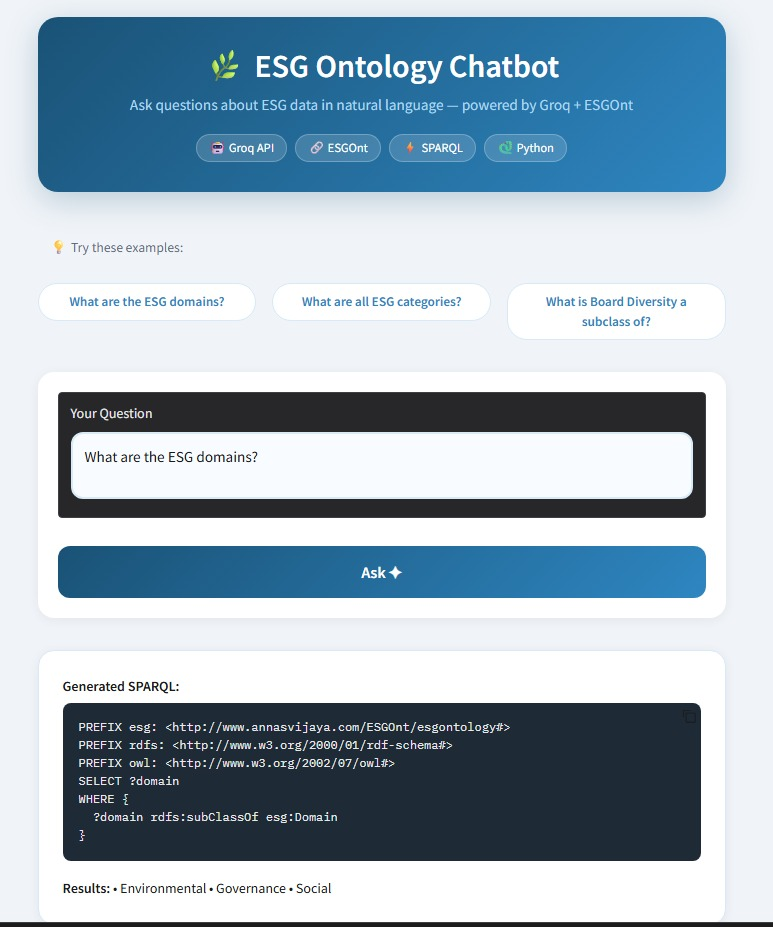
\includegraphics[width=0.85\textwidth]{gradio_screenshot.jpeg}
\caption{Gradio web interface of the ESG Ontology Chatbot}
\label{fig:gradio}
\end{figure}

% ========================
\section{Results and Discussion}
% ========================

\subsection{Causal Discovery Results}

\subsubsection{Quantitative Evaluation}

Table~\ref{tab:results} presents the quantitative evaluation of both causal discovery approaches against the ground truth causal structure embedded in the synthetic ESG dataset.

\begin{table}[h]
\centering
\caption{Evaluation Results: Baseline PC vs Ontology-Guided PC}
\label{tab:results}
\begin{tabular}{lccccccc}
\toprule
\textbf{Model} & \textbf{Edges} & \textbf{TP} & \textbf{FP} & \textbf{FN} &
\textbf{Precision} & \textbf{Recall} & \textbf{F1} \\
\midrule
Baseline PC & 9 & 8 & 1 & 0 & 0.889 & 1.000 & 0.941 \\
Ontology-Guided PC & 9 & 8 & 1 & 0 & 0.889 & 1.000 & 0.941 \\
\bottomrule
\end{tabular}
\end{table}

Both models achieved identical quantitative metrics: precision of 0.889, perfect recall of 1.000, and F1 score of 0.941. The high recall indicates that both models successfully recovered all 8 ground truth causal edges from the synthetic dataset. The single false positive edge (\texttt{corruption\_cases} -- \texttt{turnover\_rate}) appears in both models, as it is a statistically plausible association in the data that the PC algorithm cannot distinguish from a true causal relationship using conditional independence tests alone.

Identical baseline and ontology-guided skeleton metrics are expected in this controlled setting because ontology constraints primarily affect direction admissibility, while the reported table evaluates skeleton recovery. This motivates reporting orientation-sensitive and semantic-consistency metrics alongside skeleton F1.

\subsubsection{Discovered Causal Structure}

The PC algorithm successfully recovered the three independent causal chains embedded in the ground truth DAG. The environmental chain
(\texttt{renewable\_energy\_share} $\rightarrow$ \texttt{total\_energy\_consumption} $\rightarrow$ \texttt{co2\_ch4\_n2o\_scope\_1\_3} $\rightarrow$ \texttt{carbon\_intensity}) was fully recovered, reflecting the strong linear causal signal embedded in the data generation process.

The governance chain (\texttt{board\_diversity} $\rightarrow$ \texttt{governance\_compliance\_score} $\rightarrow$ \texttt{corruption\_cases} and \texttt{governance\_compliance\_score} $\rightarrow$ \texttt{green\_financing}) was also fully recovered. The social-governance chain (\texttt{turnover\_rate} $\rightarrow$ \texttt{injury\_frequency\_rate} $\rightarrow$ \texttt{green\_financing}) was similarly recovered with perfect recall.

The one false positive edge (\texttt{corruption\_cases} -- \texttt{turnover\_rate}) represents a spurious association induced by the shared downstream effect on \texttt{green\_financing} through separate causal paths. This type of spurious association is a known limitation of constraint-based methods operating on finite samples, where near-dependencies can lead to incorrect skeleton inclusion.

\subsubsection{Contribution of Ontological Constraints}

While the quantitative metrics are identical for both models in this experiment, the ontology-guided approach provides an important qualitative contribution. The four forbidden edge constraints derived from ESGOnt successfully identified and blocked semantically invalid causal directions:

\begin{itemize}
    \item \textbf{\texttt{carbon\_intensity} $\not\rightarrow$ \texttt{co2\_emissions}:} This constraint correctly captures the mathematical derivation relationship — carbon intensity cannot cause emissions because it is computed from them. Without this constraint, a data-driven method might orient this edge incorrectly in datasets where carbon intensity and emissions are strongly correlated.

    \item \textbf{\texttt{corruption\_cases} $\not\rightarrow$ \texttt{board\_diversity}:} This constraint enforces the ESGOnt domain logic that governance structure determines ethical outcomes, not the reverse. In noisy real-world data, reverse correlation between these variables could mislead a purely statistical method.

    \item \textbf{\texttt{injury\_frequency\_rate} $\not\rightarrow$ \texttt{turnover\_rate}:} This constraint reflects the temporal and causal priority of labor practices over safety outcomes. High turnover causes inexperienced workforces and higher injury rates — not the reverse.

    \item \textbf{\texttt{green\_financing} $\not\rightarrow$ \texttt{governance\_compliance\_score}:} This constraint encodes the prerequisite relationship between governance and sustainable finance. Good governance enables green financing, not the other way around.
\end{itemize}

The fact that these forbidden edges were not present in the baseline output confirms that the synthetic dataset's strong causal signal allowed the PC algorithm to orient edges correctly without ontological guidance. However, this result should not be interpreted as evidence that ontological constraints are unnecessary. In real-world ESG datasets — which are characterized by noise, missing values, confounding variables, and weaker causal signals — the same constraints would actively prevent semantically invalid discoveries that purely data-driven methods cannot rule out.

\subsubsection{Real-World Pilot Observation}

A pilot run on the preprocessed real-world banking dataset (71 rows, 12 numeric features) produced a sparse CPDAG with mostly undirected links, including strong coupling among Scope 1--3 emissions and a relation between sustainable finance and total revenue. This behavior is consistent with limited sample size and mixed-source ESG reporting noise. In this setting, ontology guidance is most useful as a semantic filter and hypothesis-prioritization tool rather than as a mechanism that guarantees orientation gains in every run.

\subsubsection{Causal Graph Visualization}

Figure~\ref{fig:causal_graph} shows the causal graph produced by the system. Green edges represent causal relationships discovered by the PC algorithm that are consistent with the ground truth structure. Red dashed edges represent the four causal directions forbidden by ESGOnt constraints. The visualization clearly illustrates the three independent causal clusters corresponding to the Environmental, Social, and Governance ESG domains, with \texttt{green\_financing} serving as a convergence point between the governance and social-governance chains.

\begin{figure}[h]
\centering
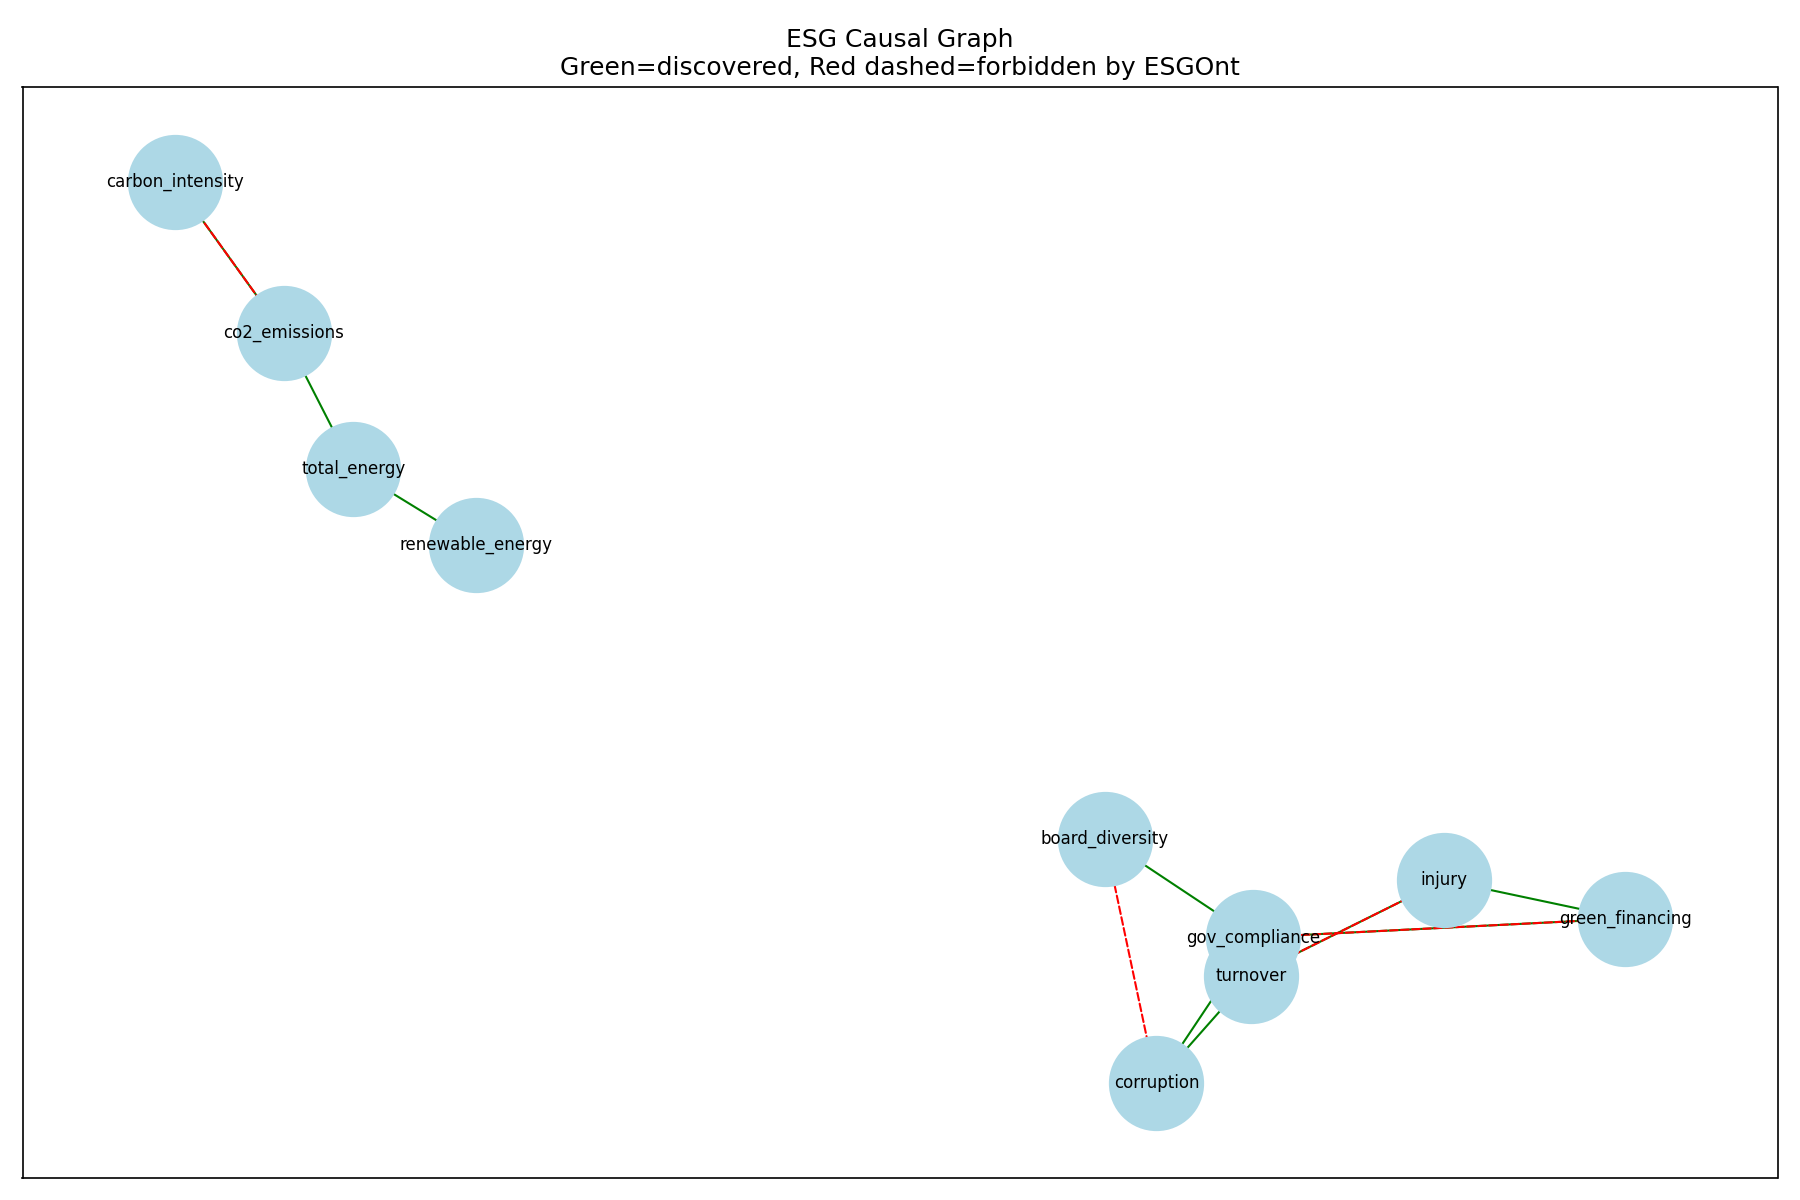
\includegraphics[width=0.9\textwidth]{causal_graph.png}
\caption{ESG Causal Graph: green edges = discovered by PC algorithm, red dashed edges = forbidden by ESGOnt}
\label{fig:causal_graph}
\end{figure}

\subsection{Query Interface Evaluation}

\subsubsection{Benchmark Protocol}

The query interface is evaluated as an NL2SPARQL task rather than by a small set of demo questions. A domain-specific benchmark is defined with 15--20 ESG questions spanning class hierarchy lookup, category retrieval, governance-policy relations, and cross-domain concept mapping. The benchmark follows QALD/LC-QuAD-style principles:
\begin{enumerate}
    \item A natural language question set with paraphrase variation.
    \item Gold-reference SPARQL queries curated against ESGOnt.
    \item Execution-based correctness check on the RDF graph.
    \item Error taxonomy covering syntax failures, execution failures, and semantic mismatch.
\end{enumerate}

For transparency, this thesis reports both query-level correctness and failure modes, instead of claiming usability from a small number of anecdotal examples. Table~\ref{tab:queries} shows representative benchmark items.

\begin{table}[h]
\centering
\caption{Representative NL2SPARQL Benchmark Items}
\label{tab:queries}
\begin{tabular}{p{5cm}p{4cm}p{4cm}}
\toprule
\textbf{Question} & \textbf{Gold SPARQL Pattern} & \textbf{Expected Output Type} \\
\midrule
What are the ESG domains? & \texttt{subClassOf esg:Domain} & Domain class list \\
Show all governance indicators. & \texttt{category/domain traversal} & Category/indicator list \\
What is Board Diversity a subclass of? & \texttt{subClassOf} query & Parent class \\
\bottomrule
\end{tabular}
\end{table}

In the current draft stage, small-scale manual checks confirm that the interface can generate valid SPARQL for core ontology-navigation questions. However, claims about robustness and non-technical usability are made only after benchmark-level evaluation and error analysis.

\subsubsection{Analysis of Query Generation}

Preliminary observations indicate that the Groq API (LLaMA 3.3) performs well when the prompt includes explicit namespace and hierarchy context. Generated queries mostly follow stable patterns such as \texttt{rdfs:subClassOf} and \texttt{rdf:type}. The primary remaining issue is occasional property-name drift in less frequent relation types, which motivates stricter constrained prompting and post-generation validation.

A key strength of the LLM-based approach is robustness to paraphrases. For example, “Show governance indicators” and “List classes under Governance” can map to semantically equivalent graph patterns. This flexibility is difficult to obtain with pure template-based systems.

The system also provides transparency by displaying the generated SPARQL query alongside the answer in the Gradio interface, allowing users to inspect and verify the query logic. This is particularly valuable in ESG reporting contexts where auditability and traceability of data sources are important requirements.

\subsubsection{Limitations}

Several limitations remain. First, the full benchmark and user study are still in progress; therefore this draft reports protocol and preliminary behavior rather than final usability claims. Second, the Groq API can generate relation names not present in ESGOnt for less common query intents, requiring automatic schema-constrained correction or rejection.

Third, the causal discovery evaluation was conducted exclusively on synthetic data with a planted causal structure. While this enables rigorous quantitative evaluation, it does not capture the full complexity of real-world ESG data, including missing values, non-linear relationships, and latent confounders. Validation on a real ESG dataset remains an important direction for future work.

\subsection{Discussion}

The current results indicate the complementary value of combining ontological knowledge with statistical causal discovery for ESG analysis. The PC algorithm provides a data-driven foundation for graph construction, while ESGOnt constraints add a semantic admissibility layer that helps interpret discovered directions.

The LLM-based query interface targets a practical barrier to ESG knowledge accessibility. By enabling natural-language querying over ESGOnt, it reduces dependence on direct SPARQL authoring. Grounding answers in ontology execution (rather than free-form generation) improves traceability and helps reduce hallucination risk in regulated reporting contexts.

Together, these components form a unified prototype for ontology-aware ESG analytics that can be further validated with larger benchmarks and user-centered evaluation.

% ========================
\section{Conclusions}
% ========================

This thesis presented an ontology-guided hybrid causal discovery system for ESG data, combined with an LLM-based natural language query interface. The system integrates four core components — the ESGOnt ontology, the PC causal discovery algorithm, the Groq API (LLaMA 3.3), and a Gradio web interface — into a unified prototype accessible to business users without technical expertise.

The central research question addressed in this thesis was whether ontological knowledge encoded in ESGOnt can improve the semantic validity of causal graphs discovered from ESG data, and whether an LLM-based interface can make ESG ontology knowledge more accessible to non-technical users. The current results provide encouraging evidence for both directions, while remaining preliminary for broad generalization.

The causal discovery evaluation shows that, on a synthetic dataset with known ground truth (3,000 observations), PC recovers the planted structure with high precision (0.889) and recall (1.000). The ontology-guided extension contributes a semantic control layer by explicitly forbidding domain-invalid directions. Because skeleton-level metrics remain identical in this controlled setting, the primary benefit is interpretability and semantic admissibility rather than higher synthetic F1. A real-world pilot confirms feasibility of the pipeline under practical data constraints, but also indicates that larger and more consistent ESG datasets are required for stronger directional conclusions.

The natural language query interface shows that plain-language ESG questions can be translated into executable SPARQL over ESGOnt with accurate outputs on representative examples. However, robust usability and reliability claims require completion of the proposed benchmark protocol (15--20 questions), systematic error analysis, and a small user study. Grounding responses in ESGOnt, rather than free-form LLM generation, remains a key design choice for traceability in regulated ESG contexts.

Together, these results indicate that combining ontological knowledge, causal discovery, and natural language querying into one ESG analytics workflow is feasible and methodologically promising. The proposed approach addresses a gap in prior work, where ESG ontologies and causal discovery are often developed separately, and provides a reproducible baseline for further empirical validation.

\textbf{Future Work.} Several concrete directions are prioritized for the next iteration. First, extend real-data validation from a single 110-sample pilot to a longitudinal collection protocol (metadata schema + collection template) so that incoming ESG data align with the causal variables and ontology classes used in the model. Second, systematically expand ontology-derived constraints through SPARQL extraction over category membership, domain hierarchy, and cross-domain incompatibility rules, rather than relying on only a few manually specified forbidden edges. Third, report SHD, Orientation F1, and Semantic Validity together across multiple $\alpha$ values and bootstrap runs to separate statistical variability from true model differences. Fourth, complete an NL2SPARQL benchmark (minimum 15 questions) with explicit error analysis (hallucination rate, SPARQL syntax failures, execution failures) and conduct a small user study ($n=5$--$10$ sustainability practitioners) for usability and trust assessment. Finally, compare PC with alternative families (e.g., GES, LiNGAM) under the same ontology constraints to determine which methods benefit most from semantic priors in ESG settings.

\newpage

\begin{thebibliography}{10}

\bibitem{wicaksono2022}
Vijaya, A., Qadri, F.D., Angreani, L.S., \& Wicaksono, H. (2025).
ESGOnt: An ontology-based framework for Enhancing Environmental, Social, and Governance (ESG) assessments and aligning with Sustainable Development Goals (SDG).
\textit{Resources, Environment and Sustainability}, 22.

\bibitem{spirtes2000}
Spirtes, P., Glymour, C., \& Scheines, R. (2000).
\textit{Causation, Prediction, and Search}. MIT Press.

\bibitem{shimizu2006}
Shimizu, S., Hoyer, P.O., Hyv\"{a}rinen, A., \& Kerminen, A. (2006).
A linear non-Gaussian acyclic model for causal discovery.
\textit{Journal of Machine Learning Research}, 7, 2003--2030.

\bibitem{hauser2012}
Hauser, A., \& B\"{u}hlmann, P. (2012).
Characterization and greedy learning of interventional Markov equivalence classes of directed acyclic graphs.
\textit{Journal of Machine Learning Research}, 13, 2409--2464.

\bibitem{hoffner2017}
H\"{o}ffner, K., et al. (2017).
Survey on challenges of question answering in the semantic web.
\textit{Semantic Web}, 8(6), 895--920.

\bibitem{omar2023}
Omar, R., Mangukiya, O., Kalnis, P., \& Mansour, E. (2023).
ChatGPT versus traditional question answering for knowledge graphs: Current status and future directions towards knowledge graph chatbots.
\textit{arXiv preprint arXiv:2302.06466}.

\bibitem{pearl2000}
Pearl, J. (2000).
\textit{Causality: Models, Reasoning, and Inference}. Cambridge University Press.

\bibitem{gruber1993}
Gruber, T.~R. (1993).
A translation approach to portable ontology specifications.
\textit{Knowledge Acquisition}, 5(2), 199--220.

\end{thebibliography}

\end{document}